% ============================================================================
% NanoBubbleEval: NeurIPS 2026 Evaluations & Datasets Track
% Draft v0.5: multi-task benchmark for schema extraction, numerical
% grounding, and evidence attribution in scientific information extraction,
% instantiated on the nanobubble / nanocarrier literature.
% ============================================================================

\documentclass{article}
\usepackage[eandd]{neurips_2026}
\usepackage{amsmath,amssymb,amsfonts}
\usepackage{booktabs}
\usepackage{graphicx}
\usepackage{hyperref}
\usepackage{multirow}
\usepackage{xcolor}
\usepackage{enumitem}
\usepackage{array}
\usepackage{longtable}
\usepackage{makecell}
\usepackage{tabularx}
\usepackage{ragged2e}
\usepackage[most]{tcolorbox}
\usepackage[T1]{fontenc}
\usepackage[utf8]{inputenc}
\usepackage{textcomp}
\usepackage{lmodern}
\usepackage{xurl}
\usepackage{rotating}

\definecolor{nbblue}{RGB}{36,99,167}
\definecolor{nbred}{RGB}{198,80,80}
\definecolor{nbteal}{RGB}{30,150,140}
\definecolor{nbsoftblue}{RGB}{244,249,255}
\definecolor{nbsoftred}{RGB}{255,247,247}
\definecolor{findingbg}{RGB}{246,249,246}
\definecolor{findingbar}{RGB}{30,110,60}

\newtcolorbox{findingbox}[1]{%
  enhanced, breakable,
  colback=findingbg, colframe=findingbar,
  leftrule=3.5pt, rightrule=0.5pt, toprule=0.5pt, bottomrule=0.5pt,
  arc=2pt, left=8pt, right=7pt, top=6pt, bottom=6pt,
  title=#1, coltitle=white, fonttitle=\bfseries\small,
}

\newcommand{\NR}{\texttt{NOT\_REPORTED}}

\title{NanoBubbleEval: An Evidence-Grounded Benchmark for Schema Extraction,
Numerical Grounding, and Evidence Attribution in the Nanobubble and
Nanocarrier Literature}

\author{
Elias Hossain \\
\texttt{anonymous@anonymous}
}

\begin{document}
\maketitle

% ============================================================================
\begin{abstract}
Nanobubble and nanocarrier research spans biomedical delivery, imaging, environmental remediation, agriculture, and colloidal physics, yet its quantitative findings remain scattered across paper text, tables, and figures. We introduce \textbf{NanoBubbleEval}\footnote{Dataset: \url{https://huggingface.co/datasets/EliasHossain/nanobubbleeval}. Code: \url{https://github.com/eliashossain001/nanobubbleeval}.}, to our knowledge the first abstract-level structured benchmark and reproducible evaluation scaffold for nanobubble and nanocarrier extraction. v1.0 is positioned as a \emph{seed} benchmark: it pairs a 51{,}566-record deduplicated warehouse (of which approximately 81.7\% contain abstracts) with a 40-record gold-hard seed evaluation tier annotated under an 18-field schema, together with the harvest-to-evaluation pipeline that produced them. The high-precision core, the full 500-record gold pool, and the 460-record gold-lite extension tier are scheduled for v1.1 and are regenerable from the included pipeline scripts; no headline v1.0 claim depends on them. The evaluation protocol defines three task views over the gold-hard tier -- schema extraction, unit-normalised numerical grounding, and verbatim evidence attribution -- with the standalone task-view CSV files also scheduled for v1.1. We benchmark rule-based extraction, BioBERT-SQuAD-v2, and Qwen2.5-7B-Instruct using three domain-aligned metrics: abstention-calibrated F1, tolerance-bounded numerical match, and answer--evidence consistency. Qwen2.5-7B-Instruct achieves the best macro abstention-calibrated F1 (0.758), ahead of BioBERT-SQuAD-v2 (0.545) and rule-based extraction (0.493), but shows reduced robustness on review abstracts and lower evidence consistency than span-based extractors. We treat these numbers as seed-tier diagnostics rather than a definitive ranking. NanoBubbleEval contributes a deterministic harvest-to-evaluation pipeline, slice annotations, leakage auditing, a recovery audit trail (\texttt{verification/}), Croissant 1.1 metadata, and an open-source Python evaluation harness, establishing reproducible infrastructure on which the community can extend the seed.
\end{abstract}


\section{Introduction}
\label{sec:intro}

Nanobubble and nanocarrier research has grown into a flourishing, cross-disciplinary field, with annual publication volume rising more than an order of magnitude over the past two decades (Fig.~\ref{fig:publication_volume}). Yet its quantitative findings -- hydrodynamic size, zeta potential, stability, encapsulated payload, loading efficiency, release kinetics -- remain scattered across paper bodies, tables, and figures, with no structured community resource. Adjacent fields have solved this problem at the resource layer: the Materials Project~\citep{jain2013materials}, the Protein Data Bank~\citep{berman2000pdb}, and ChEMBL~\citep{gaulton2012chembl} have each been transformative for their domains. Nanobubble and nanocarrier research has no analogous resource.

\begin{figure}[t]
\centering
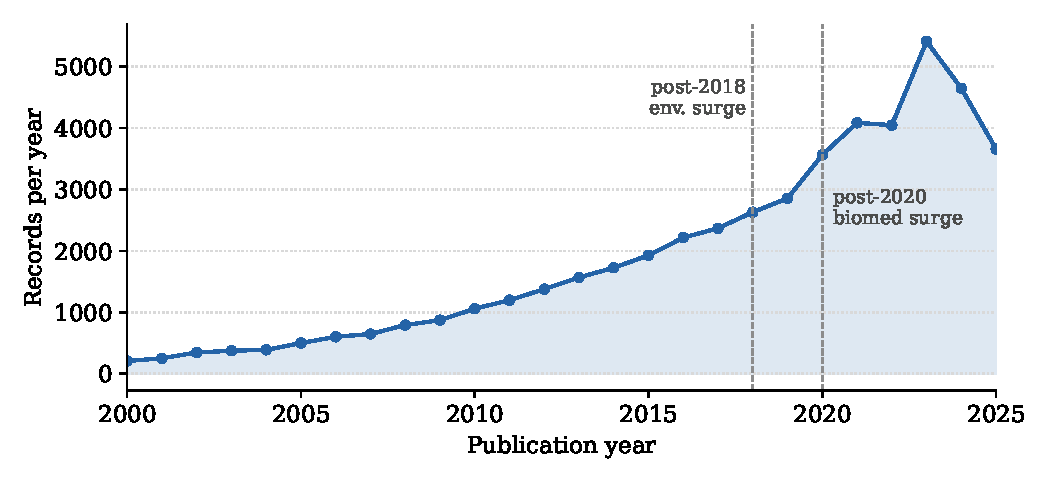
\includegraphics[width=0.78\columnwidth]{figs/publication_volume.pdf}
\caption{Annual publication volume in the \textit{NanoBubbleEval} warehouse, 2000--2025 ($n{=}49{,}340$). The post-2018 surge is driven primarily by environmental and water-treatment applications; the post-2020 acceleration adds biomedical drug delivery and ultrasound contrast imaging. The field is flourishing, but no structured resource exists to consolidate its quantitative findings.}
\label{fig:publication_volume}
\end{figure}

This paper introduces \textit{NanoBubbleEval}, to our knowledge the first abstract-level structured benchmark for nanobubble and nanocarrier extraction, together with a reproducible evaluation scaffold for it. The v1.0 release is intentionally seed-scale: a 51{,}566-record deduplicated warehouse paired with a 40-record gold-hard seed evaluation tier and three reference baselines, framed as a starting point the community can extend rather than a fully mature benchmark. The 18-field schema, harvest-to-evaluation pipeline, unit-normalisation tables, metric suite, and recovery audit are released together; the benchmark in this paper establishes the scoring protocol on the seed tier and surfaces the three failure modes the metric suite is designed to detect.

Existing scientific information-extraction benchmarks evaluate parts of this problem -- span- and entity-level QA~\citep{jain2020scirex,islamaj2021nlmchem,li2016bc5cdr,jin2019pubmedqa}, schema-based property extraction~\citep{dunn2022matscholar,song2023matscinlp,zaki2023mascqa}, and evidence-grounded factuality~\citep{wadden2020scifact,lu2023scitab} -- but none target nanobubble and nanocarrier literature, and none jointly stress the three failure modes that govern reliable population of a structured resource in a sparse, unit-heavy, evidence-sensitive scientific domain.

\paragraph{Contributions.}
We make four contributions:

\begin{itemize}\itemsep0pt

\item \textbf{Seed benchmark for nanobubble and nanocarrier literature.}
v1.0 establishes a reproducible seed evaluation tier and release pipeline: a 51{,}566-record deduplicated warehouse (released in v1.0) and a 40-record gold-hard seed evaluation tier, instantiating an 18-field schema. The 8{,}006-record high-precision core, the 500-record gold pool, the 460-record gold-lite extension tier, and the three task-view CSVs are scheduled for v1.1 and are regenerable from the released scripts; no headline v1.0 claim depends on them.

\item \textbf{Domain-fitted evaluation scaffold.}
Three task views (schema extraction, unit-normalised numerical grounding, verbatim evidence attribution) and three metrics (\emph{abstention-calibrated F1}, \emph{tolerance-bounded numerical match}, \emph{answer--evidence consistency}) that target the specific failure modes of sparse, unit-bearing, evidence-sensitive extraction in this literature, packaged as an open-source Python evaluation harness.

\item \textbf{Reference baselines on the seed tier.}
Three reference baselines spanning rule-based extraction, biomedical extractive QA, and instruction-tuned generation, scored on the gold-hard seed tier under a blind, abstract-only protocol with single-annotator-validated labels. The baseline numbers are seed diagnostics, not a definitive ranking.

\item \textbf{Diagnostic findings that motivate v1.1 work.}
The instruction-tuned baseline reaches macro abstention-calibrated F1 of $0.758$ versus $0.545$ and $0.493$ for the extractive-QA and rule-based floors, but drops $33.7$ points on review abstracts versus original-research abstracts and is the only baseline whose answer--evidence consistency falls below $1.000$. We surface these as diagnostics that point to concrete improvements (better review-abstract handling, evidence-constrained decoding) and motivate the v1.1 scope rather than treat them as final claims.

\end{itemize}

% % ============================================================================
% \section{Related Work}
% \label{sec:related}

% Scientific information-extraction benchmarks fall into three broad
% families, each capturing a different facet of the problem. We
% position NanoBubbleEval against each family below; domain-specific
% nanobubble physics literature, which motivates the schema design but
% not the NLP framing, is summarised in Appendix~\ref{app:domain_background}.

% \paragraph{Span and entity QA.}
% SciREX~\citep{jain2020scirex}, BC5CDR~\citep{li2016bc5cdr},
% NLM-Chem~\citep{islamaj2021nlmchem}, and
% PubMedQA~\citep{jin2019pubmedqa} evaluate mention recognition or
% single-answer QA on biomedical and scientific text. These resources
% are well-suited to entity-level NLP, but they do not test joint
% numerical grounding or treat abstention as a first-class output, so a
% model that fabricates plausible spans and a model that cites
% unsupported evidence are scored equivalently.

% \paragraph{Schema-constrained property extraction.}
% Matscholar~\citep{dunn2022matscholar},
% MatSci-NLP~\citep{song2023matscinlp},
% MaScQA~\citep{zaki2023mascqa}, and recent
% LLM-based property extraction~\citep{polak2023extracting} evaluate
% JSON-shaped or table-shaped outputs against a fixed schema. They
% share NanoBubbleEval's structured-output framing but typically credit
% any non-empty value uniformly, with no metric that penalises emission
% where the source is silent.

% \paragraph{Evidence-grounded factuality.}
% SciFact~\citep{wadden2020scifact}, SciTab~\citep{lu2023scitab}, and
% recent retrieval-augmented evaluation
% frameworks~\citep{ru2024ragchecker} score whether a claim is
% \emph{supported} by retrieved evidence. These resources address one
% of our three failure modes (evidence attribution) but do not assess
% the quantitative correctness of a claim under unit normalisation, and
% they do not catch the case where the answer is correct but the cited
% span does not contain it.

% \paragraph{How NanoBubbleEval differs.}
% NanoBubbleEval departs from this prior work along four axes. First,
% three structured tasks share a single record set, which lets us
% decompose failure modes \emph{within} an example rather than compare
% performance across heterogeneous benchmarks. Second, an explicit
% \NR{} convention is scored under abstention-calibrated F1, which
% distinguishes a correct abstain from an incorrect emission. Third,
% unit-normalised numerical match isolates unit drift from value drift.
% Fourth, an answer-evidence consistency rate catches
% cite-hallucination, in which the answer is correct but the cited span
% does not contain it, as a first-class failure rather than folding it
% into a span F1. We make no claim that v1.0 matches the annotation
% depth of expert-curated single-task benchmarks; instead, we position
% v1.0 as a structured \emph{multi-task} benchmark anchored by
% a stratified gold-hard tier produced under a pre-specified blind
% dual-annotator protocol (v1.0 ships single-annotator-validated
% labels; full dual annotation is planned for v1.1), with explicitly
% declared abstract-only scope.

% ============================================================================
% ============================================================================
\section{Related Work}
\label{sec:related}

Existing scientific information-extraction benchmarks address parts of the problem in isolation. Span- and entity-level QA~\citep{jain2020scirex,li2016bc5cdr,islamaj2021nlmchem,jin2019pubmedqa} target mention recognition, relation extraction, or single-answer QA without jointly evaluating abstention, unit normalisation, and evidence faithfulness. Schema-constrained property-extraction benchmarks~\citep{dunn2022matscholar,song2023matscinlp,zaki2023mascqa,polak2023extracting} evaluate JSON- or table-shaped outputs against fixed schemas but typically credit any non-empty prediction uniformly, making it hard to distinguish valid extraction from unsupported schema filling. Evidence-grounded factuality benchmarks~\citep{wadden2020scifact,lu2023scitab,ru2024ragchecker} score support but do not test numerical correctness under unit normalisation or detect cases where a correct answer is paired with an unsupported span.

\paragraph{Structured resources in nanobubble and nanocarrier research.}
Adjacent fields have community resources that consolidate primary literature into machine-readable form: the Materials Project~\citep{jain2013materials}, the Protein Data Bank~\citep{berman2000pdb} (which underpins AlphaFold~\citep{jumper2021highly}), and ChEMBL~\citep{gaulton2012chembl}. Nanobubble and nanocarrier research has no analogous resource: quantitative findings (size, surface charge, stability, payload, loading efficiency, release profile) are reported per-paper in heterogeneous formats. Building this resource through automated extraction requires both a structured target schema and an evaluation harness rigorous enough to trust the extracted values; \textit{NanoBubbleEval} contributes both.

\paragraph{Positioning of \textit{NanoBubbleEval}.}
\textit{NanoBubbleEval} addresses these gaps by treating sparse, unit-bearing, evidence-sensitive scientific extraction as a unified problem rather than as separate subtasks, and by anchoring the evaluation in a concrete domain that lacks structured infrastructure. Unlike prior span-level, schema-based, or evidence-grounded benchmarks, \textit{NanoBubbleEval} defines three task views over the same record set: schema extraction with \NR{} as a first-class output, unit-normalized numerical grounding, and verbatim evidence attribution. This design makes it possible to isolate schema-fill hallucination, unit or value drift, and cite-hallucination within the same examples. The resulting framework is not intended to replace expert-curated single-task benchmarks; it provides the validation harness that lets the community trust automated population of the underlying structured resource.




% % ============================================================================
% % Domain Background relocated to Appendix~\ref{app:domain_background}.

% % ============================================================================
% \section{Task and Schema}
% \label{sec:task}

% We frame nanobubble property extraction as a multi-task structured
% prediction problem over a shared schema. Given a record $r$ with
% title $t_r$ and abstract $a_r$, NanoBubbleEval defines three
% evaluation views over an 18-field normalised schema $\mathcal{S}$.
% Six fields are designated \emph{headline} because abstract-level
% coverage supports reliable per-field reporting on the gold-hard
% tier; the remaining twelve are \emph{provisional} and retained
% for schema stability and forward compatibility
% (Table~\ref{tab:schema_scope}). Three task views are projected from
% the same gold-pool annotation pass, which lets us attribute errors
% to specific failure modes for the same example.

% \paragraph{Task 1: structured extraction.} Given $a_r$, predict
% $\hat{V}=\{\hat{v}_f : f \in \mathcal{S}\}$, where each $\hat{v}_f$
% is either a normalised value or \NR{}. Scored by per-field
% exact-match F1 and by abstention-calibrated F1
% (\S\ref{sec:metrics}).

% \paragraph{Task 2: numerical grounding.} Given $a_r$ and a target
% field $f$ with a numeric type, predict
% $(\hat{x}_f, \hat{u}_f)$, the numeric value and its normalised unit.
% Scored by tolerance-bounded match on $\hat{x}_f$ after unit
% normalisation, with unit accuracy reported as a separate axis to
% disentangle unit drift from value drift.

% \paragraph{Task 3: evidence attribution.} Given $a_r$, $f$, and the
% predicted answer, return a verbatim span $\hat{e}_f$ of $a_r$ that
% supports the answer (or \NR{}). Scored by character-set IoU against
% the gold span and by an \emph{answer-evidence consistency rate}, the
% fraction of records in which a correct $\hat{v}_f$ is paired with a
% span that contains the value.

% \begin{table}[t]
% \centering
% \caption{v1.0 schema scope. Headline fields carry sufficient
% abstract-level coverage to support reliable reporting on the
% gold-hard tier; provisional fields are retained for schema
% stability and future releases. Coverage values are the proportion of
% records in the 52{,}519-record warehouse with a positive heuristic
% flag for the field.}
% \label{tab:schema_scope}
% \small
% \setlength{\tabcolsep}{6pt}
% \begin{tabular}{@{}p{0.46\columnwidth}p{0.46\columnwidth}@{}}
% \toprule
% \textbf{Headline (6 fields)} & \textbf{Provisional (12 fields)} \\
% \midrule
% \texttt{size} (26.3\%)              & \texttt{generation\_method} (23.3\%) \\
% \texttt{zeta\_potential} (6.5\%)    & \texttt{characterization\_method} (24.0\%) \\
% \texttt{stability} (19.8\%)         & \texttt{material\_identity} \\
% \texttt{payload} (55.4\%)           & \texttt{bubble\_type} \\
% \texttt{loading\_efficiency} (19.0\%) & \texttt{application\_category} \\
% \texttt{release\_profile} (24.6\%)  & \texttt{medium\_environment} \\
%                                     & \texttt{outcome\_claim} \\
%                                     & \texttt{evidence\_span} \\
%                                     & \texttt{ambiguity\_flag} \\
%                                     & three additional unit slots \\
% \bottomrule
% \end{tabular}
% \end{table}

% \paragraph{Why \NR{} is a first-class output.}
% A naive scoring rule that compares emitted values to gold values
% without distinguishing absence from emission penalises a model that
% correctly abstains and rewards a model that fabricates a plausible
% value. In abstract-derived extraction over a sparse domain like
% nanobubble characterisation, where on average only $2.4$ of the six
% headline fields are reported per abstract on the 40-record gold
% slice, this conflation systematically overstates extractor quality. Abstention-calibrated F1
% (\S\ref{sec:metrics}) credits a correct \NR{} as a true positive on a
% \emph{distinct} class, separating schema-fill hallucination from
% genuine extraction skill.

% ============================================================================
% Domain Background relocated to Appendix~\ref{app:domain_background}.

% ============================================================================
\section{Task and Schema}
\label{sec:task}

We frame property extraction as multi-task structured prediction over an 18-field schema $\mathcal{S}$. Six fields are designated \emph{headline} (sufficient abstract-level coverage for reliable seed-tier reporting); the remaining twelve are \emph{provisional} and retained for schema stability (Table~\ref{tab:schema_scope}). All three task views derive from the same gold-pool annotation pass, allowing errors to be compared across tasks for the same record.
\textbf{Task 1 (Structured extraction)}: predict $\hat{V}=\{\hat{v}_f : f \in \mathcal{S}\}$ with $\hat{v}_f \in V_f \cup \{\NR{}\}$; scored by per-field exact-match F1 and abstention-calibrated F1.
\textbf{Task 2 (Numerical grounding)}: for each numeric field, predict $(\hat{x}_f, \hat{u}_f)$; scored by tolerance-bounded numerical match after canonical-unit conversion, with unit accuracy reported separately.
\textbf{Task 3 (Evidence attribution)}: predict a verbatim span $\hat{e}_f$ that supports $\hat{v}_f$, or \NR{}; scored by character-set IoU and an \emph{answer--evidence consistency} rate (fraction of correct predictions whose span contains the value).

\begin{table}[t]
\centering
\caption{v1.0 schema scope. Headline fields have sufficient abstract-level coverage for reliable reporting on the gold-hard tier. Provisional fields are retained for schema stability and future releases. Coverage values indicate the proportion of records in the 51{,}566-record warehouse with a positive heuristic flag for the field.}
\label{tab:schema_scope}
\small
\setlength{\tabcolsep}{6pt}
\begin{tabular}{@{}p{0.46\columnwidth}p{0.46\columnwidth}@{}}
\toprule
\textbf{Headline (6 fields)} & \textbf{Provisional (12 fields)} \\
\midrule
\texttt{size} (26.3\%)              & \texttt{generation\_method} (23.3\%) \\
\texttt{zeta\_potential} (6.5\%)    & \texttt{characterization\_method} (24.0\%) \\
\texttt{stability} (19.8\%)         & \texttt{material\_identity} \\
\texttt{payload} (55.4\%)           & \texttt{bubble\_type} \\
\texttt{loading\_efficiency} (19.0\%) & \texttt{application\_category} \\
\texttt{release\_profile} (24.6\%)  & \texttt{medium\_environment} \\
                                    & \texttt{outcome\_claim} \\
                                    & \texttt{evidence\_span} \\
                                    & \texttt{ambiguity\_flag} \\
                                    & three additional unit slots \\
\bottomrule
\end{tabular}
\\[2pt]
{\footnotesize Coverage values denote heuristic detection rates over warehouse records and do not represent gold-validated reporting frequencies.}
\end{table}

\paragraph{\NR{} as an abstention signal.}
Correct abstention is essential in this benchmark because many abstracts do not report every target property. A naive metric that only compares emitted values against gold values can penalize a model that correctly abstains and can fail to distinguish unsupported emissions from valid extractions. This issue is especially important in nanobubble and nanocarrier abstracts, where only a subset of the six headline fields is usually reported. In the 40-record gold-hard slice, each abstract reports an average of only $2.4$ headline fields. Treating \NR{} as a distinct output class allows abstention-calibrated F1 (\S\ref{sec:experimental_setup}) to reward correct non-emission and to separate genuine extraction ability from schema-fill hallucination.

% ============================================================================
\section{Benchmark Construction}
\label{sec:construction}

\textit{NanoBubbleEval} is constructed through a five-stage pipeline (warehouse harvest, tier curation, gold-pool sampling, annotation, task-view projection); the released code reconstructs every stage end-to-end from the source APIs.

\paragraph{Warehouse harvesting.}
We collect abstracts and metadata from PubMed (NCBI Entrez), Europe PMC, OpenAlex, CrossRef, Semantic Scholar, and ClinicalTrials.gov v2 across five query families (nanobubble core; ultrasound and contrast imaging; delivery and release; biomedical nanocarriers; environmental and agricultural applications). Records are deduplicated in a fixed order: DOI, PMID/PMCID, normalized title, URL. The released v1.0 warehouse contains \textbf{51{,}566 deduplicated records}, of which 81.7\% include abstracts (Table~\ref{tab:warehouse_stats}); OpenAlex contributes $50{,}022$ records and PubMed $1{,}544$. Europe PMC, CrossRef, Semantic Scholar, and ClinicalTrials.gov are wired into the framework but contribute zero post-deduplication records to v1.0; their independent expansion ships with v1.1.

\paragraph{Provenance and gold-hard integrity.}
The v1.0 warehouse is a 2026-05 re-harvest produced after a project-deletion incident destroyed the 2026-03 warehouse from which the gold-hard tier was sampled. We re-anchor the warehouse to the gold-hard records by direct identifier lookup: each gold-hard \texttt{record\_id} encodes a canonical source-API identifier (12 PubMed DOIs, 27 OpenAlex DOIs, one Europe PMC DOI). The 2026-05 re-harvest already contained 26 of the 40 records; the remaining 14 were re-fetched by direct DOI lookup and merged in under the original gold-hard \texttt{record\_id}. The annotation-time abstract is preserved verbatim in the warehouse for every re-fetched row, so baseline predictions remain exactly reproducible. The warehouse is therefore a strict superset of the gold-hard tier ($40/40$ resolve directly). The full identifier-anchored recovery audit (\texttt{verification/}, shipped in v1.0) contains the parsed identifiers, before/after-merge containment tables, the re-fetch log, an abstract cross-check (14 verbatim, 19 Unicode/whitespace-normalised, 7 source-side editorial revisions), and a machine-readable \texttt{summary.json}.

\paragraph{Tier curation and high-precision core.}
Warehouse records are tier-labelled by lexical proximity to nanobubble-related terms; A1 records contain explicit nanobubble terminology and A2 records contain adjacent ultrasound or gas-carrier vocabulary. The \textbf{high-precision core} (A1+A2) contains 8{,}006 records (3{,}577 A1, 4{,}429 A2) and is the candidate source for benchmark sampling. The core CSV ships with v1.1; the tier rules and pipeline ship with v1.0.

\paragraph{Gold pool and seed evaluation tier.}
From the high-precision core, a 500-record \textbf{gold pool} is sampled balanced by nanobubble-vs-nanoparticle label, document type, and field coverage. The gold pool is partitioned into a 40-record \textbf{gold-hard seed evaluation tier} (stratified by \texttt{nb\_label} $\times$ \texttt{document\_type}; blind, abstract-only dual-annotator protocol; v1.0 ships single-annotator-validated labels) and a 460-record \textbf{gold-lite tier} (single-annotator; constructed for internal robustness; dev=50, test=410). v1.0 makes no headline claim that depends on the gold-lite tier or the gold pool itself; both ship with v1.1 alongside the high-precision core.

\begin{table}[t]
\centering
\caption{Layered counts of the benchmark construction pipeline. The
warehouse and the gold-hard tier ship in v1.0; the high-precision
core, candidate pool, gold pool, and gold-lite tier are constructed
internally by the released pipeline and are scheduled for v1.1.
The gold-hard tier follows a dual-annotator protocol; v1.0 reports
single-annotator-validated labels. The gold-lite tier is single-annotator
and used only for internal robustness analysis.}
\label{tab:warehouse_stats}
\small
\setlength{\tabcolsep}{6pt}
\begin{tabular}{@{}lrll@{}}
\toprule
\textbf{Layer} & \textbf{Records} & \textbf{Notes} & \textbf{Release} \\
\midrule
Warehouse (deduplicated)        & 51{,}566 & 81.7\% with abstracts          & v1.0 \\
\quad OpenAlex                  & 50{,}022 & dominant source                & v1.0 \\
\quad PubMed                    &  1{,}544 & secondary source               & v1.0 \\
High-precision core (A1+A2)     &  8{,}006 & 3{,}577 A1, 4{,}429 A2         & v1.1 \\
Benchmark candidate pool        &  1{,}000 & balanced sample                & v1.1 \\
Gold pool                       &    500 & gold-hard + gold-lite            & v1.1 \\
\quad Gold-hard tier            &     40 & headline evaluation              & v1.0 \\
\quad Gold-lite tier            &    460 & dev=50, test=410                 & v1.1 \\
\bottomrule
\end{tabular}
\end{table}

\paragraph{Evaluation slices.}
Each gold-pool record is assigned five slice tags for stratified analysis: year bucket, source API, document type, nanobubble-vs-nanoparticle label, and application bucket (Table~\ref{tab:slice_summary}). The year buckets are pre-2015, 2015--2020, and post-2020. The application buckets include biomedical, environmental, fundamental, industrial, and other. Slices with fewer than 30 total records are reported only in the appendix to avoid unstable per-slice estimates.

\begin{table}[t]
\centering
\caption{Slice membership in the gold pool ($n=500$). Slices marked (\emph{apx}) contain fewer than five gold-hard records and are reported only in the appendix.}
\label{tab:slice_summary}
\small
\setlength{\tabcolsep}{4pt}
\begin{tabular}{@{}lrrrr@{}}
\toprule
\textbf{Slice value} & \textbf{Total} & \textbf{Gold-Hard} & \textbf{Gold-Lite Dev} & \textbf{Gold-Lite Test} \\
\midrule
\multicolumn{5}{@{}l}{\emph{Nanobubble vs.\ nanoparticle}} \\
\quad nanobubble                & 197 & 18 & 20 & 159 \\
\quad nanoparticle              & 251 & 16 & 26 & 209 \\
\quad micro/nanobubble          &  39 &  3 &  4 &  32 \\
\quad microbubble-adjacent (\emph{apx}) &  13 &  3 &  0 &  10 \\
\midrule
\multicolumn{5}{@{}l}{\emph{Document type}} \\
\quad original                  & 390 & 32 & 39 & 319 \\
\quad review                    & 110 &  8 & 11 &  91 \\
\midrule
\multicolumn{5}{@{}l}{\emph{Year bucket}} \\
\quad post-2020                 & 296 & 19 & 31 & 246 \\
\quad 2015--2020                & 150 & 17 & 16 & 117 \\
\quad pre-2015                  &  54 &  4 &  3 &  47 \\
\midrule
\multicolumn{5}{@{}l}{\emph{Application bucket}} \\
\quad biomedical                & 365 & 28 & 35 & 302 \\
\quad environmental             & 117 & 12 & 12 &  93 \\
\quad fundamental (\emph{apx})  &  11 &  0 &  2 &   9 \\
\bottomrule
\end{tabular}
\end{table}

\paragraph{Task-view construction.}
The 500 gold records are deterministically projected into three evaluation views (the standalone task-view CSV files are scheduled for v1.1; v1.0 evaluates the three views directly on the 40-record gold-hard tier). The structured extraction view requires a complete schema fill. The numerical grounding view is restricted to numeric headline fields and includes value, unit, and tolerance specifications. The evidence attribution view requires a verbatim supporting span for each emitted field. Because all three views originate from the same annotation pass, differences across task scores reflect model behavior rather than inconsistencies across separate gold datasets.


% % ============================================================================
% \section{Dataset Release and Artifact Organization}
% \label{sec:release}

% The v1.0 release is organised into a Python package, a layered data
% release, and an evaluation harness. The package
% (\texttt{nanobubbleval}) implements the schema, the unit normaliser,
% the dev/test split builder, the inter-annotator reconciler, the
% evaluator, and a baseline interface; subclasses of the baseline
% abstract class plug into the same evaluation harness without
% modification. The data release is structured by lifecycle stage: a
% deduplicated warehouse manifest, the high-precision nanobubble core,
% the gold pool with its five-slice annotations, the three task views
% described above, the 40-record gold-hard subset with first-annotator
% labels, and a Croissant 1.1 metadata file populated with the
% NeurIPS-required responsible-AI fields.

% We additionally release the annotation guideline used for the IAA
% subset, the deterministic split files (with a leakage-audit report
% verifying disjointness across splits), and the four numbered
% pipeline scripts that reproduce every artifact end-to-end from a
% clean checkout. A complete listing of release artifacts and their
% canonical locations is provided in
% Appendix~\ref{app:release_card}.

% \begin{itemize}\itemsep0pt
% \item \textbf{Code} (Python package and pipeline scripts): \\
% \url{https://github.com/eliashossain001/nanobubbleeval}
% \item \textbf{Dataset} (gold pool, gold-hard tier, baseline
% predictions, schema specification, and Croissant 1.1 metadata): \\
% \url{https://huggingface.co/datasets/EliasHossain/nanobubbleeval}
% \end{itemize}

% The release is licensed for research use under terms detailed in
% \S\ref{sec:limitations}. The first-annotator gold-hard labels are
% released alongside the gold pool to allow downstream users to
% recompute agreement statistics against their own annotators and to
% apply their own match policies; full multi-annotator adjudication is
% planned for v1.1.

% ============================================================================
\section{Dataset Release and Artifact Organization}
\label{sec:release}

The v1.0 release ships a Python package (\texttt{nanobubbleval}: schema, unit normalization, splits, reconciliation, evaluator, and baseline interface), a layered dataset bundle, and an evaluation harness shared by all baselines. Table~\ref{tab:release_status} summarises which artifacts are released today and which are regenerable from the pipeline and scheduled for v1.1; Appendix~\ref{app:release_card} expands the list to file paths.

\begin{itemize}\itemsep0pt
\item \textbf{Code:} \url{https://github.com/eliashossain001/nanobubbleeval}
\item \textbf{Dataset:} \url{https://huggingface.co/datasets/EliasHossain/nanobubbleeval}
\end{itemize}

\begin{table}[h]
\centering
\caption{v1.0 release-status summary. The artifacts in the upper block are
released on HuggingFace today and carry every headline claim in this paper.
The lower block is regenerable end-to-end from the released pipeline scripts
and is scheduled for v1.1; no v1.0 headline claim depends on it.}
\label{tab:release_status}
\small
\setlength{\tabcolsep}{4pt}
\renewcommand{\arraystretch}{1.15}
\begin{tabularx}{\linewidth}{@{}p{0.30\linewidth} c X p{0.20\linewidth}@{}}
\toprule
\textbf{Artifact} & \textbf{v1.0?} & \textbf{Role in current claims} & \textbf{Planned extension} \\
\midrule
51{,}566-record warehouse manifest    & Yes & Corpus construction, gold-hard containment & Live re-harvest (v1.2+) \\
18-field schema (\texttt{configs/extraction\_schema.json}) & Yes & Drives all evaluation                       & Schema v2 (v1.1) \\
40-record gold-hard seed tier         & Yes & All headline metrics                        & Dual annotation (v1.1) \\
Baseline predictions (B1, B2, B3)     & Yes & Reproducibility of Table~\ref{tab:headline_results} & Larger ceiling + RAG variants (v1.1) \\
Leakage and recovery audits (\texttt{verification/}, \texttt{splits/}) & Yes & Validity of provenance and split & Updated audits per release \\
\midrule
8{,}006-record high-precision core; 500-record gold pool; 460-record gold-lite extension tier; three task-view CSVs; \texttt{splits.json} & v1.1 & \emph{Not used for any v1.0 headline claim} & Ships in v1.1; regenerable from the released pipeline scripts \\
\bottomrule
\end{tabularx}
\end{table}

The code and dataset are released for research use (see \S\ref{sec:limitations}); first-annotator gold-hard labels support independent re-scoring and alternative match policies, and full multi-annotator adjudication is planned for v1.1.

% % ============================================================================
% \section{Validity Safeguards}
% \label{sec:validity}

% A 500-record gold pool is small relative to expert-curated single-task
% benchmarks, so v1.0 supports its evaluation claims through five
% explicit safeguards rather than through scale alone.

% \paragraph{Schema and unit normalisation.}
% Every emitted value is validated against the 18-field schema, and
% every numeric field is normalised to a canonical unit (nm for size,
% mV for zeta potential, hours for stability, percent for loading
% efficiency) before scoring. Out-of-vocabulary unit strings are
% flagged but never silently coerced, so unit drift surfaces explicitly
% in the metric tables rather than being absorbed into a single
% correctness score.

% \paragraph{Gold-hard tier ($n=40$, dual-annotator protocol).}
% A 40-record subset, stratified by
% \texttt{nb\_label} $\times$ \texttt{document\_type}, is annotated
% under a pre-specified blind, abstract-only protocol on the six
% headline fields. v1.0 ships
% \emph{single-annotator-validated labels under the dual-annotator
% protocol}: the first-annotator pass (an external biomedical
% annotator) is complete and is what headline numbers are scored
% against; full dual annotation and inter-annotator agreement
% statistics (Cohen's $\kappa$ on \NR{}-versus-emit, character-set
% span IoU on emit-emit pairs, and unit-normalised exact-match on
% numeric fields) are planned for the v1.1 release.
% Table~\ref{tab:iaa_summary} documents the planned IAA-reporting
% schema. The first-annotator labels are released alongside the gold
% pool so that downstream users can recompute agreement statistics
% against their own annotators under their own match policies.

% \paragraph{Adjudication, scope, and reproducibility.}
% Adjudication is defined by protocol (disagreements resolved by the
% first author under a logged decision rule once the second-annotator
% pass completes; v1.0 uses single-annotator-validated labels on the
% gold-hard tier). v1.0 evaluates exclusively on abstracts: properties
% stated only in tables, methods, or supplementary material are out of
% scope, and \NR{} is the correct answer even when the underlying
% paper reports the value. The dev/test split is constructed
% deterministically with a fixed seed; the split file, slice-membership
% map, and a leakage-audit report are released. Full details for all
% three safeguards are in Appendix~\ref{app:pipeline}.

% ============================================================================
\section{Validity Safeguards}
\label{sec:validity}

The seed-scale gold-hard tier ($n=40$) is supported by four explicit safeguards. \textbf{Schema and unit normalization.} All predictions are validated against the 18-field schema before scoring; numeric fields are converted to canonical units (nm, mV, h, \%), and out-of-vocabulary units are flagged rather than silently coerced. \textbf{Annotation status.} v1.0 reports single-annotator-validated labels from an external biomedical annotator under a pre-specified blind, abstract-only dual-annotator protocol; full dual annotation and IAA statistics are planned for v1.1, and the released first-annotator labels allow downstream users to apply alternative matching policies. \textbf{Scope.} v1.0 evaluates abstract-derived extraction only; values reported only in full text, tables, or supplementary material are out of scope and \NR{} is the correct label. \textbf{Reproducibility.} The dev/test split is deterministic (seed=42); slice and leakage-audit reports ship in v1.0, while the per-record \texttt{splits.json} is regenerable from the released scripts and ships in v1.1 (Appendix~\ref{app:pipeline}).



% % ============================================================================
% \section{Method and Baselines}
% \label{sec:method}

% We benchmark three baseline families that span rule-based, encoder,
% and instruction-LLM approaches. All three consume the abstract and
% emit predictions for the six headline fields under a single prompt
% or pattern set; no baseline is given access to the document's full
% text. Together they bound a wide range of contemporary extraction
% strategies and reveal where each strategy fails.

% \paragraph{B1: Regex baseline.}
% Hand-written regular expressions for each numeric headline field
% (\texttt{size}, \texttt{zeta\_potential}, \texttt{stability},
% \texttt{loading\_efficiency}). Patterns match number-unit pairs in
% the immediate textual neighbourhood of field-indicative anchor
% phrases, with negative lookarounds that reject ranges and
% uncertainty markers. The baseline returns \NR{} when no pattern
% matches. The two non-numeric fields (\texttt{payload} and
% \texttt{release\_profile}) are returned as \NR{} by B1, since regex
% extraction over abstracts is too noisy for free-text fields.

% \paragraph{B2: BioBERT QA-span (SQuAD-v2).}
% \texttt{ktrapeznikov/biobert\_v1.1\_pubmed\_squad\_v2}, a BioBERT-v1.1
% encoder fine-tuned on SQuAD-v2, is prompted with one natural-language
% question per headline field. The SQuAD-v2 unanswerable head is mapped
% directly to \NR{}; spans whose softmax-scaled confidence falls below
% $0.20$ (tuned on dev, frozen at test) are also mapped to \NR{}. We
% ship the off-the-shelf checkpoint to expose where pretrained
% biomedical extractive-QA fails without task-specific fine-tuning.

% \paragraph{B3: \texttt{Qwen2.5-7B-Instruct} (zero-shot, schema-constrained).}
% \texttt{Qwen/Qwen2.5-7B-Instruct} is prompted with the 18-field
% schema, the \NR{} convention, and one in-context worked example,
% and returns a JSON object per abstract; out-of-schema fields are
% repaired or nulled before scoring. Inference uses HuggingFace
% Transformers on a single 16\,GB GPU with greedy decoding. A
% retrieval-augmented baseline and a same-family-larger ceiling
% (\texttt{Qwen2.5-72B-Instruct}) are scheduled for v1.1.

% % ============================================================================
% \section{Metrics}
% \label{sec:metrics}

% The three task views call for three families of metrics. Each is
% chosen to expose a specific failure mode rather than to summarise
% overall correctness.

% \paragraph{Field-F1 and abstention-calibrated F1.}
% For each headline field $f$, let $y_f \in V_f \cup \{\NR{}\}$ be
% the gold value and $\hat{y}_f$ the prediction. \emph{Naive field-F1}
% computes per-class F1 over $V_f$ alone, treating both correct and
% incorrect \NR{} predictions as out-of-class. \emph{Abstention-calibrated
% F1} (Acal-F1) treats \NR{} as a distinct class and computes F1 over
% $V_f \cup \{\NR{}\}$. The Acal-F1 minus Naive-F1 gap is the
% quantitative signature of schema-fill hallucination: a model that
% fabricates values when the abstract is silent has high Naive-F1 and
% low Acal-F1, whereas a model that abstains correctly has the two
% metrics close together.

% \paragraph{Numerical match (tolerance-bounded).}
% For numeric fields, $\hat{x}_f$ is judged correct if and only if
% $|\hat{x}_f - x_f| \le \tau \cdot |x_f|$ after both values are
% mapped to canonical units, where $\tau = 0.05$ (a relative
% tolerance). We additionally report \emph{unit accuracy}
% $\mathbf{1}[\hat{u}_f = u_f]$ as a separate axis to isolate unit
% drift from value drift.

% \paragraph{Span IoU and answer-evidence consistency.}
% Evidence spans are scored by character-set IoU against the gold
% span. We additionally report an \emph{answer-evidence consistency
% rate}: the fraction of records in which a correct $\hat{v}_f$ is
% accompanied by a $\hat{e}_f$ that contains $\hat{v}_f$ as a substring.
% A model that emits the right value with a wrong span exhibits
% cite-hallucination, which the IoU metric alone does not isolate.

% ============================================================================
\section{Experimental Setup}
\label{sec:experimental_setup}

We evaluate three baselines that represent rule-based extraction, biomedical extractive QA, and instruction-tuned LLM extraction. All baselines receive only the abstract and predict the six headline fields. No baseline has access to full text, tables, methods sections, or supplementary material.

% \paragraph{Baselines.}
% \textbf{B1: Regex.} The regex baseline uses hand-written patterns for the numeric headline fields: \texttt{size}, \texttt{zeta\_potential}, \texttt{stability}, and \texttt{loading\_efficiency}. Patterns search for number-unit pairs near field-specific anchor terms. If no valid pattern is found, the model returns \NR{}. For the two free-text fields, \texttt{payload} and \texttt{release\_profile}, B1 always returns \NR{} because reliable regex extraction is not feasible for these fields.

% \textbf{B2: BioBERT QA-span.} The second baseline uses \texttt{ktrapeznikov/biobert\_v1.1\_pubmed\_squad\_v2}, a BioBERT-v1.1 encoder fine-tuned on SQuAD-v2. Each headline field is queried with a natural-language question. The SQuAD-v2 unanswerable prediction is mapped to \NR{}. Predicted spans with confidence below $0.20$ are also mapped to \NR{}; this threshold is tuned on the development set and fixed for test evaluation. This baseline measures how far an off-the-shelf biomedical extractive-QA model can go without task-specific fine-tuning.

% \textbf{B3: Qwen2.5-7B-Instruct.} The third baseline uses \texttt{Qwen/Qwen2.5-7B-Instruct} in zero-shot schema-constrained mode. The model is prompted with the 18-field schema, the \NR{} convention, and one worked example, then asked to return a JSON object for each abstract. Invalid or out-of-schema fields are repaired or set to null before scoring. Inference is performed with HuggingFace Transformers on a single 16\,GB GPU using greedy decoding. Retrieval-augmented extraction and \texttt{Qwen2.5-72B-Instruct} are left for v1.1.

\paragraph{Baselines.}
We compare three baselines of increasing capacity, all consuming the abstract only:
\textbf{B1 Regex} uses hand-written patterns for the four numeric headline fields and returns \NR{} for the two free-text fields by design.
\textbf{B2 BioBERT QA-span} uses a BioBERT-v1.1 encoder~\citep{lee2020biobert} fine-tuned on SQuAD-v2~\citep{rajpurkar2018know}; each field is queried via a natural-language question, the unanswerable head and spans with confidence $<0.20$ are mapped to \NR{} (threshold tuned on the gold-lite dev split, frozen at test).
\textbf{B3 Qwen2.5-7B-Instruct}~\citep{qwen2024qwen25} runs zero-shot schema-constrained mode, prompted with the 18-field schema, the \NR{} convention, and one worked example, returning one JSON object per abstract under greedy decoding on a single 16\,GB GPU. Retrieval-augmented and larger same-family variants are reserved for v1.1.


\paragraph{Metrics.}
We report metrics aligned with the three task views: schema extraction, numerical grounding, and evidence attribution.

For schema extraction, we report \emph{Naive field-F1} and \emph{abstention-calibrated F1} (Acal-F1). For each headline field $f$, let $y_f \in V_f \cup \{\NR{}\}$ be the gold label and $\hat{y}_f$ be the prediction. Naive field-F1 computes F1 over reported values $V_f$ only, while Acal-F1 treats \NR{} as a distinct class and computes F1 over $V_f \cup \{\NR{}\}$. The gap between Naive-F1 and Acal-F1 indicates whether a model is being rewarded for unsupported emission or correctly credited for abstention.

For numerical grounding, we evaluate numeric fields after canonical-unit conversion. A prediction $\hat{x}_f$ is counted as correct when
\[
|\hat{x}_f - x_f| \le \tau \cdot |x_f|,
\]
where $\tau = 0.05$. We also report unit accuracy, $\mathbf{1}[\hat{u}_f = u_f]$, to separate value errors from unit errors.

For evidence attribution, we score predicted evidence spans using character-set IoU against the gold span. We also report answer-evidence consistency, defined as the fraction of correct predictions whose evidence span contains the predicted value. This metric captures cite-hallucination, where the model predicts the correct answer but cites an unsupported span.

% ============================================================================
\section{Experiments}
\label{sec:experiments}

The experiments serve as a \emph{resource-validation harness}: they establish that the seed tier supports meaningful evaluation today and that the metric suite isolates the failure modes it is designed to detect. The three baselines are reference points across rule-based, extractive-QA, and instruction-tuned-generation paradigms rather than a closed-form ranking. The regex floor (B1) verifies that the schema and unit tables support deterministic numeric extraction; the BioBERT QA model (B2) verifies that the evidence-attribution view is solvable for span-based predictors; and the instruction-tuned LLM (B3) exposes non-trivial schema-extraction performance whose failure modes (Naive--Acal gap, unit accuracy, answer--evidence consistency) the metric suite records.

Reporting in v1.0 uses the 40-record gold-hard tier with first-annotator-validated labels, two paper-supported slices (nanobubble-vs-nanoparticle and document type), and three baselines. The gold-lite extension tier ($n=460$, dev=50, test=410) is single-annotator and not shipped in v1.0; no reported claim depends on it. Slices with fewer than five records are reported only in the appendix.

\subsection{Headline results on the gold-hard tier}
\label{sec:headline}

Table~\ref{tab:headline_results} reports the four headline metrics
across the three baselines on the 40-record gold-hard tier. The
Naive-Acal F1 gap is the schema-fill-hallucination signature; the
unit-accuracy column isolates unit drift from value drift; and the
answer-evidence consistency column measures the rate at which
correct values are accompanied by spans that contain them.

% \begin{table}[t]
% \centering
% \caption{Headline results on the gold-hard tier
% ($n=40$, blind, abstract-only protocol; predictions scored against
% the first-annotator labels in v1.0).
% Acal-F1 is abstention-calibrated F1; the Naive--Acal gap is the
% schema-fill-hallucination signature. Numerical match is
% tolerance-bounded ($\tau=0.05$, relative) after unit normalisation.
% Answer--Evidence (A--E) consistency is the fraction of correct values
% whose predicted span contains the value.}
% \label{tab:headline_results}
% \small
% \setlength{\tabcolsep}{4pt}
% \begin{tabular}{@{}lcccc@{}}
% \toprule
% \textbf{Baseline} & \textbf{Naive-F1} & \textbf{Acal-F1 [95\% CI]} & \textbf{Num.\ match} & \textbf{A--E consistency} \\
% \midrule
% B1 Regex                         & 0.305 & 0.493 [0.434, 0.538] & 0.889 & 1.000 \\
% B2 BioBERT QA-span (SQuAD-v2)    & 0.378 & 0.545 [0.487, 0.588] & 0.727 & 1.000 \\
% B3 Qwen2.5-7B (zero-shot)        & \textbf{0.724} & \textbf{0.758 [0.700, 0.810]} & \textbf{1.000} & 0.939 \\
% \bottomrule
% \end{tabular}
% \\[2pt]
% {\footnotesize Acal-F1 95\% bootstrap CIs computed by record-level
% resampling with replacement ($n_\mathrm{boot}=1000$, seed=42). The
% three baselines have non-overlapping CIs at the macro level.}
% \end{table}

\begin{table}[t]
\centering
\caption{Headline results on the gold-hard tier
($n=40$, blind, abstract-only protocol; predictions scored against
the first-annotator labels in v1.0). Acal-F1 is abstention-calibrated
F1; numerical match is tolerance-bounded ($\tau=0.05$) after unit
normalisation. A--E consistency is the fraction of correct values
whose predicted span contains the value.}
\label{tab:headline_results}
\small
\setlength{\tabcolsep}{3pt}
\begin{tabularx}{\columnwidth}{@{}Xcccc@{}}
\toprule
\textbf{Baseline} & \textbf{Naive-F1} & \textbf{Acal-F1 [95\% CI]} & \textbf{Num.} & \textbf{A--E} \\
\midrule
B1 Regex & 0.305 & 0.493 [0.434, 0.538] & 0.889 & 1.000 \\
B2 BioBERT QA-span & 0.378 & 0.545 [0.487, 0.588] & 0.727 & 1.000 \\
B3 Qwen2.5-7B & \textbf{0.724} & \textbf{0.758 [0.700, 0.810]} & \textbf{1.000} & 0.939 \\
\bottomrule
\end{tabularx}
\\[2pt]
{\footnotesize Num. = numerical match; A--E = answer--evidence consistency.}
\end{table}

\begin{findingbox}{Gold-hard tier summary}
On the 40-record gold-hard tier, B3 (\texttt{Qwen2.5-7B-Instruct})
achieves the highest macro Acal-F1 ($0.758$), outperforming B2
BioBERT QA-span ($0.545$) and B1 Regex ($0.493$). All three baselines
reach perfect unit accuracy on emit-emit pairs, suggesting that most
errors come from deciding whether and what to extract rather than from
unit conversion. However, B3 has lower answer--evidence consistency
($0.939$ vs.\ $1.000$ for B1 and B2), showing that stronger extraction
can introduce cite-hallucination, especially for free-text fields such
as \texttt{payload} and \texttt{release\_profile}. Because B1 and B2
are span-based or pattern-based systems, their perfect answer--evidence
consistency partly reflects architectural constraints, whereas B3 can
generate values not explicitly grounded in its predicted span. B2
performs best on \texttt{stability}, indicating that span-based QA
remains effective for short, directly stated answers.
\end{findingbox}

\subsection{Slice Analysis}
\label{sec:slices}

Tables~\ref{tab:slice_nb} and~\ref{tab:slice_doc} report macro Acal-F1 by particle label and document type. The largest gap is by document type: B3 drops from $0.786$ on original-research abstracts to $0.449$ on review abstracts, a $33.7$-point decrease, while B1 and B2 drop only $12.6$ and $15.6$ points. Review abstracts paraphrase values rather than state them directly. The nanobubble vs.\ nanoparticle slices show only small differences across baselines, suggesting no strong particle-label bias.


\begin{table}[t]
\centering
\caption{Macro Acal-F1 by particle label on the gold-hard tier. Microbubble-related slices with $n=3$ each are reported in Appendix~\ref{app:errors}.}
\label{tab:slice_nb}
\small
\setlength{\tabcolsep}{4pt}
\begin{tabular}{@{}lccc@{}}
\toprule
\textbf{Slice} & \textbf{B1 [95\% CI]} & \textbf{B2 [95\% CI]} & \textbf{B3 [95\% CI]} \\
\midrule
nanobubble ($n=18$)   & 0.491 [0.392, 0.560] & 0.549 [0.451, 0.617] & \textbf{0.765 [0.649, 0.847]} \\
nanoparticle ($n=16$) & 0.451 [0.370, 0.513] & 0.495 [0.391, 0.574] & \textbf{0.708 [0.650, 0.757]} \\
\bottomrule
\end{tabular}
\end{table}

\begin{table}[t]
\centering
\caption{Macro Acal-F1 by document type on the gold-hard tier. Bootstrap 95\% CIs are computed with record-level resampling ($n_\mathrm{boot}=1000$, seed=42).}
\label{tab:slice_doc}
\small
\setlength{\tabcolsep}{4pt}
\begin{tabular}{@{}lccc@{}}
\toprule
\textbf{Slice} & \textbf{B1 [95\% CI]} & \textbf{B2 [95\% CI]} & \textbf{B3 [95\% CI]} \\
\midrule
original ($n=32$) & 0.485 [0.428, 0.539] & 0.538 [0.484, 0.593] & \textbf{0.786 [0.727, 0.853]} \\
review ($n=8$)    & 0.359 [0.333, 0.383] & 0.382 [0.333, 0.417] & 0.449 [0.388, 0.517] \\
\midrule
\emph{drop} & $-0.126$ & $-0.156$ & $\mathbf{-0.337}$ \\
\bottomrule
\end{tabular}
\end{table}



% \subsection{Slice analysis}
% \label{sec:slices}

% Tables~\ref{tab:slice_nb} and~\ref{tab:slice_doc} report Acal-F1 by
% nanobubble-vs-nanoparticle label and by document type respectively.
% The two slices test different hypotheses: the
% nanobubble-vs-nanoparticle slice asks whether models bias toward
% nanoparticle-typical priors when given a record that describes a
% gas-filled nanobubble, and the document-type slice asks whether
% review papers (which paraphrase reported values) are easier or harder
% than original-research abstracts (which often state values directly).

% \begin{table}[t]
% \centering
% \caption{Macro Acal-F1 by nanobubble-vs-nanoparticle label on the
% gold-hard tier; the two micro-bubble slices ($n=3$ each) are
% reported only in Appendix~\ref{app:errors}.}
% \label{tab:slice_nb}
% \small
% \setlength{\tabcolsep}{4pt}
% \begin{tabular}{@{}lccc@{}}
% \toprule
% \textbf{Slice} & \textbf{B1 [95\% CI]} & \textbf{B2 [95\% CI]} & \textbf{B3 [95\% CI]} \\
% \midrule
% nanobubble ($n=18$)        & 0.491 [0.392, 0.560] & 0.549 [0.451, 0.617] & \textbf{0.765 [0.649, 0.847]} \\
% nanoparticle ($n=16$)      & 0.451 [0.370, 0.513] & 0.495 [0.391, 0.574] & \textbf{0.708 [0.650, 0.757]} \\
% \bottomrule
% \end{tabular}
% \end{table}

% \begin{table}[t]
% \centering
% \caption{Macro Acal-F1 by document type on the gold-hard tier
% (95\% bootstrap CIs in brackets; $n_\mathrm{boot}=1000$, seed=42).
% B3's $-0.337$ drop from \emph{original} ($0.786$) to \emph{review}
% ($0.449$) is the largest slice gap of any baseline; the original-
% and review-slice CIs for B3 are non-overlapping, indicating that
% the gap is robust under record-level resampling.}
% \label{tab:slice_doc}
% \small
% \setlength{\tabcolsep}{4pt}
% \begin{tabular}{@{}lccc@{}}
% \toprule
% \textbf{Slice} & \textbf{B1 [95\% CI]} & \textbf{B2 [95\% CI]} & \textbf{B3 [95\% CI]} \\
% \midrule
% original ($n=32$) & 0.485 [0.428, 0.539] & 0.538 [0.484, 0.593] & \textbf{0.786 [0.727, 0.853]} \\
% review ($n=8$)    & 0.359 [0.333, 0.383] & 0.382 [0.333, 0.417] & 0.449 [0.388, 0.517] \\
% \midrule
% \emph{drop (point)} & $-0.126$ & $-0.156$ & $\mathbf{-0.337}$ \\
% \bottomrule
% \end{tabular}
% \end{table}

% The most informative slice gap is on document type. B3's macro
% Acal-F1 falls from $0.786$ on original-research abstracts to $0.449$
% on review-paper abstracts, a $33.7$-point drop on a baseline that
% otherwise dominates the rule-based and encoder floors. B1 drops by
% $12.6$ points and B2 by $15.6$ points on the same slice, indicating
% that the LLM is more than twice as sensitive to review-paper
% paraphrase as the simpler baselines. The gap reflects a structural
% difference in how the two document types report quantitative
% properties: original abstracts state values directly, whereas review
% abstracts paraphrase or aggregate values across cited studies, often
% without anchoring each value to a specific particle population. The
% nanobubble-vs-nanoparticle gap is small ($+0.06$ Acal-F1 in favour of
% nanobubble for B3 on $n=18$ versus $n=16$, and similar for B1 and B2),
% suggesting that none of the three baselines exhibits a strong
% nanoparticle prior on this benchmark. The two micro-bubble slices
% ($n=3$ each) are reported only in the appendix; their counts are too
% small to support per-slice F1 estimates.



\subsection{Construct Validity on the Gold-Hard Tier}
\label{sec:iaa_eval}

v1.0 headline results are scored against first-annotator labels under a pre-specified blind, abstract-only protocol designed for dual annotation (Appendix~\ref{app:guideline}). v1.1 will report Cohen's $\kappa$ on the \NR{}-versus-emit decision, character-set span IoU on emit-emit evidence pairs, and unit-normalised exact match on numeric fields; the released first-annotator labels let downstream users recompute agreement statistics against their own annotators or apply alternative match policies.


% % ============================================================================
% \section{Limitations and Ethics}
% \label{sec:limitations}

% \paragraph{Single-domain instantiation.}
% v1.0 is instantiated on the nanobubble and nanocarrier literature.
% The schema, the metric suite, and the harvest-to-evaluation pipeline
% are domain-portable, but the lexical patterns and unit-normalisation
% tables that ship with v1.0 are calibrated to this domain; headline
% numbers should not be extrapolated to other materials-science or
% biomedical extraction domains without re-validation. The release ships
% the schema and unit-normaliser as a Python package so that downstream
% users can adapt the methodology to new domains.

% \paragraph{Abstract-only scope.}
% v1.0 evaluates abstract-derived extraction. Properties stated only in
% tables, methods, or supplementary material are out of scope, and
% \NR{} is the correct answer under our scoring rule even when the
% underlying paper reports the value. The numerical grounding task is
% bounded by abstract-level coverage; the v1.1 release will extend to
% an open-access full-text gold subset under an unchanged schema.

% \paragraph{Two-tier annotation.}
% The v1.0 gold-hard tier ($n=40$) is single-annotator-validated
% under a pre-specified blind dual-annotator protocol; full dual
% annotation and inter-annotator agreement statistics are planned for
% v1.1. The gold-lite extension tier ($n=460$, dev=50, test=410) is
% single-annotator and reported only as a robustness check. Headline
% claims are scored on the gold-hard tier exclusively. We do not claim
% multi-expert adjudication for v1.0.

% \paragraph{Baseline scope.}
% v1.0 benchmarks three rule-based and open-weights baselines and does
% not evaluate proprietary frontier models. We make no comparative
% claim about closed-API model behaviour on this benchmark; v1.1 will
% add a same-family-larger ceiling (\texttt{Qwen2.5-72B-Instruct})
% following the protocol of \citet{lu2023scitab}, plus a
% retrieval-augmented baseline over open-access full text.

% \paragraph{Ethics and licensing.}
% All warehouse records are sourced from public scholarly APIs under
% their respective terms; the release preserves DOIs and PMIDs and
% redistributes only derived structured curation. The release ships a
% Croissant 1.1 metadata file with the NeurIPS-required responsible-AI
% fields. The benchmark contains no human subjects, no identifiable
% medical records, and no patient-level information. The codebase is
% released under the MIT license; the dataset is released for
% non-commercial research use under terms documented in the release.

% ============================================================================
\section{Limitations and Ethics}
\label{sec:limitations}

\textit{NanoBubbleEval} v1.0 is limited to nanobubble and nanocarrier abstracts. Although the schema, metrics, and pipeline are domain-portable, the lexical filters and unit-normalization rules are calibrated to this literature and should be re-validated before use in other domains. The benchmark is abstract-only: values appearing only in full text, tables, methods, or supplementary materials are out of scope, and \NR{} is correct when the abstract does not state the property. The baseline set covers regex extraction, biomedical extractive QA, and one open-weights instruction model, but excludes proprietary and retrieval-augmented full-text systems. All records come from public scholarly APIs; the release redistributes derived structured annotations only, contains no human-subject or patient-level data, and is released for non-commercial research use.

\paragraph{Seed-tier limitations.}
v1.0 is positioned as a transparent seed benchmark, not a definitive ranking. (i) $n{=}40$ is sufficient for seed validation of the metric suite and surfacing failure modes, but not for a final leaderboard; the non-overlapping bootstrap CIs in Table~\ref{tab:headline_results} should be read as distinguishable seed regimes. (ii) Slice-stratified results (Table~\ref{tab:slice_nb}, Table~\ref{tab:slice_doc}) are diagnostic rather than conclusive: with $n{=}3$ on the smallest slices and $n{=}8$ on review abstracts, slice gaps highlight directions for further work. (iii) Released first-annotator labels support reproducibility and alternative match policies, but final dual-annotator adjudication and Cohen's $\kappa$ / span-IoU statistics remain future work for v1.1. (iv) v1.0 is abstract-only by construction; full-text grounding ships in v1.1 alongside the high-precision core, gold pool, gold-lite tier, and task-view CSVs.


% ============================================================================
\section{Conclusion}
\label{sec:conclusion}

\textit{NanoBubbleEval} is, to our knowledge, the first abstract-level structured benchmark and reproducible evaluation scaffold for nanobubble and nanocarrier literature. It instantiates an 18-field schema on a 51{,}566-record warehouse paired with a 40-record gold-hard seed evaluation tier, three reference baselines, and the harvest-to-evaluation pipeline (Table~\ref{tab:release_status}). The high-precision core, 500-record gold pool, gold-lite tier, and task-view CSVs are regenerable from the released scripts and ship in v1.1. Three baselines surface the failure modes the metric suite is designed to detect: schema-fill hallucination on free-text fields, a $33.7$-point drop on review abstracts versus original-research abstracts, and the first observed cite-hallucination once an extractor moves beyond span-based prediction. \textit{NanoBubbleEval} provides reproducible infrastructure for seed-scale evaluation and extension, and invites the community to build on the directions in our v1.1 roadmap (\S\ref{sec:roadmap}).

% ============================================================================
\section{v1.1 Roadmap}
\label{sec:roadmap}

v1.0 is intentionally scoped to be defensible end-to-end; the roadmap below converts the deferred work into a research programme.
\begin{itemize}\itemsep0pt
\item \textbf{Full dual annotation on the gold-hard tier} -- complete the second-annotator pass on all 40 records under the v1.0 protocol and report Cohen's $\kappa$, span IoU, and unit-normalised exact match.
\item \textbf{Community expansion of the seed tier} -- release the 500-record gold pool (gold-hard $\cup$ 460-record gold-lite extension) and adjudicate gold-lite subsets into gold-hard status, with a standing pull-request workflow for community annotations.
\item \textbf{Open-access full-text grounding} -- extend the benchmark to an open-access full-text gold subset under the same schema, evaluating extraction from tables and figures under the same metric suite.
\item \textbf{Frontier and retrieval-augmented baselines} -- add a same-family-larger ceiling (\texttt{Qwen2.5-72B-Instruct}), a proprietary frontier API, and a retrieval-augmented variant over open-access full text.
\item \textbf{Cross-domain portability} -- instantiate the schema, unit tables, and metric suite on at least one adjacent materials-science or biomedical-extraction domain.
\end{itemize}

% ============================================================================
\section*{Impact Statement}
\label{sec:impact}

\textit{NanoBubbleEval} exposes three failure modes (schema-fill hallucination, unit drift, cite-hallucination) and discourages downstream systems from using unsupported values in literature review, database construction, and meta-analysis. Two risks remain. First, gold-hard results should not be extrapolated to other materials-science or biomedical domains without re-validation; downstream pipelines should preserve the abstention and evidence-provenance signals. Second, the warehouse is dominated by English-language abstracts from a limited set of scholarly APIs, biasing coverage toward English biomedical and environmental publications. We mitigate by releasing the schema, unit tables, evaluation harness, and curation procedures, and by semantically versioning the benchmark so that v1.1 (multi-rater adjudication, full-text grounding) does not invalidate v1.0 results.

% ============================================================================
\section*{AI Use Statement}
\label{sec:ai_use_statement}

\texttt{Qwen2.5-7B-Instruct} is evaluated as the B3 baseline (\S\ref{sec:experimental_setup}) -- a research subject, not a generation tool. \textit{NanoBubbleEval} itself is constructed without LLMs: harvesting, deduplication, tier curation, sampling, slice tagging, and the metric suite are deterministic and rule-based; the schema and annotation guideline were authored by human contributors. AI-assisted writing tools were used during code drafting, LaTeX formatting, and editorial refinement; all scientific claims, experimental measurements, gold annotations, baseline implementations, and final wording were reviewed and approved by the authors. No AI tool generated the gold-hard annotations, computed the reported metrics, or authored the empirical conclusions.


% ============================================================================
\bibliographystyle{plainnat}
\bibliography{ref}

% ============================================================================
\clearpage
\appendix
\renewcommand\thesection{\Alph{section}}
\renewcommand\thesubsection{\thesection.\arabic{subsection}}

\label{sec:final-appendix}
\addcontentsline{toc}{section}{Supplementary Material}
\tableofcontents

\newpage

\section{Domain background}
\label{app:domain_background}

The schema design is informed by the structure of the nanobubble
literature. Two partly distinct lines of work shape the field:
nanobubbles as interfacial or bulk physicochemical entities whose
persistence challenges classical dissolution theory, and nanobubbles
as engineered carriers in water treatment, agriculture, ultrasound
imaging, and drug delivery.

\subsection{Foundational studies on observation and stability.}
Atomic force microscopy studies reported nanoscale gas domains on
hydrophobic surfaces and characterised their behaviour at solid--water
interfaces \citep{Lou2000NanobubblesSolid,Tyrrell2001ImagesNanobubbles,Zhang2008NanobubblesInterface,Borkent2007SuperstabilitySurface}.
Bulk nanobubbles introduce a related challenge: their stability
requires a physicochemical explanation involving gas--liquid
interfaces, charge, and solution chemistry
\citep{Ohgaki2009PhysicochemicalApproach,Jadhav2020BulkNanobubbles,Tan2020BulkNanobubbles,Zhou2021GenerationStability,Tan2021StabilitySurface}.
Surface and bulk systems differ in generation, measurement, and
interpretation, motivating the schema separation of
\texttt{generation\_method}, \texttt{characterization\_method}, and
\texttt{bubble\_type}.

\subsection{Generation and characterisation.}
Generation methods (periodic pressure variation, ceramic membrane
filtration, ultrasonication, Henry's-law approaches, electric-field
generation) strongly influence size distribution, concentration, gas
composition, and stability
\citep{Wang2019GenerationStability,Ahmed2018GenerationNanobubbles,Yasuda2018GenerationReduction,Ferraro2020HenryMethod,Ghaani2020MassiveGeneration},
and characterisation across instruments and assumptions yields
non-comparable measurements
\citep{Zhang2020ExperimentalStudy,Zhou2020UltrahighDensity,Li2021BulkNanobubbles,Meegoda2019ApplicationDiffused}.
NanoBubbleEval encodes both as first-class schema fields.

\subsection{Application domains.}
Environmental and water engineering applications include water and
wastewater treatment, aeration, contaminant removal, membrane
processes, ecological restoration, mineral processing, and adsorption
\citep{Jia2023NanobubblesWater,Zhou2022UntappedPotential,Azevedo2019BulkNanobubbles,Kyzas2018NanobubblesEffect}.
Agricultural applications cover gas-specific nanobubbles for seed
germination, plant growth, and crop productivity
\citep{Ahmed2018InfluencesOxygen,Wu2019EnhancementTomato,Wang2021NanobubblesPromote}.
Biomedical applications use nanobubbles as stimulus-responsive
carriers, ultrasound-active agents, or oxygen-delivery platforms,
requiring schema attributes such as \texttt{payload},
\texttt{loading\_efficiency}, and \texttt{release\_profile}
\citep{Xiong2021StimuliResponsive,Su2021CurrentAdvances,Batchelor2020NestedNanobubbles,Song2020BiogenicNanobubbles,DuanL2020MicroNano}.

\subsection{Why a structured benchmark is needed.}
Existing reviews summarise parts of the field
\citep{Zhou2021GenerationStability,Tan2021StabilitySurface,Jia2023NanobubblesWater,Xiong2021StimuliResponsive}
but do not provide a structured dataset suitable for model
evaluation. NanoBubbleEval converts publicly available abstracts into
structured records under a uniform schema, enabling the three-task
benchmarking methodology presented in the main paper.

\section{Error taxonomy}
\label{app:error_taxonomy}

To make headline numbers actionable, we hand-inspect a sample of B3
errors and classify each into one of five recurring categories. The
taxonomy is intentionally small: each category corresponds to a
metric that can detect it programmatically, so future systems can be
diagnosed against the same axes without additional human labour.

\begin{itemize}\itemsep0pt
\item \textbf{Schema-fill hallucination.} The model emits a value
when the abstract states nothing. Detected by the
Acal-F1-minus-Naive-F1 gap.
\item \textbf{Unit drift.} The numeric value is correct but the unit
is wrong (for example, \texttt{200}\,\textmu{}m for a record that
reports \texttt{200}\,nm). Detected by the unit-accuracy column.
\item \textbf{Entity--value mis-binding.} The value is correct for
some property in the abstract but is assigned to the wrong field
(for example, binding a loading-efficiency value to release
profile).
\item \textbf{Cite-hallucination.} The value is correct but the
predicted span does not contain it. Detected by the answer-evidence
consistency rate.
\item \textbf{Topic confusion (nanobubble vs.\ nanoparticle).} The
model applies nanoparticle-typical priors (for example, assuming a
polymer matrix) on a record that describes a gas-filled nanobubble.
Cross-checked against the nanobubble-vs-nanoparticle slice gap.
\end{itemize}

Representative worked examples for B3 are included in
Appendix~\ref{app:errors}. Additional examples across the full gold
pool will be released with v1.1.

\section{Pipeline details}
\label{app:pipeline}

\paragraph{Harvest query families.}
The 51{,}566-record warehouse is harvested across five query
families, each instantiated as a set of keyword expressions issued to
the public scholarly APIs listed in \S\ref{sec:construction}.

\begin{itemize}\itemsep0pt
\item \emph{Nanobubble core} -- nanobubble; bulk nanobubble; ultrafine
bubble; micro nanobubble; oxygen nanobubble; nanobubble stability;
nanobubble characterisation; nanobubble generation; nanobubble
cavitation; nanobubble imaging; nanobubble therapy; nanobubble drug
delivery.
\item \emph{Ultrasound and contrast imaging} -- ultrasound contrast
agent; gas-filled liposome; acoustic nanocarrier; targeted ultrasound
imaging; molecular ultrasound imaging; ultrasound-triggered drug
delivery; sonodynamic therapy nanocarrier; theranostic ultrasound
nanoparticle.
\item \emph{Delivery and release} -- nanoparticle payload; loading
efficiency; encapsulation efficiency; release profile; controlled
release nanoparticle; sustained release nanocarrier; drug loading
nanoparticle; carrier stability; colloidal stability; particle size
zeta potential.
\item \emph{Biomedical nanocarriers} -- lipid nanoparticle drug
delivery; polymer nanoparticle delivery; liposome drug loading;
cubosome drug delivery; niosome drug delivery; exosome-coated
nanocarrier; PLGA nanoparticle release; targeted cancer nanocarrier;
nanomedicine; nanocarrier; drug delivery system; controlled release;
biomedical nanocarrier.
\item \emph{Environmental, water, and agriculture} -- nanobubble
water treatment; micro nanobubble irrigation; oxygen nanobubble
aquaculture; nanobubble flotation; nanobubble biofilm removal;
nanobubble wastewater treatment; nanobubble agriculture.
\end{itemize}

\paragraph{Deduplication order.}
Records are merged across APIs in strict order: DOI first, then
PMID/PMCID, then normalised title, then URL. Title normalisation
lowercases, removes punctuation and stop-tokens, and collapses
whitespace; the leakage-audit report confirms
that no \texttt{record\_id} appears in more than one split.

\paragraph{Tier rules.}
Records are assigned to Tier A, B, or C based on lexical proximity
to the nanobubble-core vocabulary in title and abstract. Tier A is
further split: A1 records contain at least one explicit
\emph{nanobubble} or \emph{ultrafine bubble} surface form; A2 records
contain adjacent ultrasound or gas-carrier vocabulary
(\emph{microbubble}, \emph{contrast agent}, \emph{gas-filled
liposome}). The high-precision core (8{,}006 records) is the union
of A1 and A2; B and C records are retained in the warehouse for
coverage but excluded from benchmark candidate sampling.

\paragraph{Benchmark candidate sampling.}
A 1{,}000-record candidate pool is drawn from the high-precision
core, balanced across the nanobubble-vs-nanoparticle label, document
type, and field-coverage signals (heuristic flags for
\texttt{size}, \texttt{zeta\_potential}, \texttt{stability},
\texttt{payload}, \texttt{loading\_efficiency},
\texttt{release\_profile}). The 500-record gold pool is the
top-ranked half of the candidate pool by an
extraction-priority score that rewards records with multiple
field-coverage flags. The dev/test split is constructed
deterministically with seed=42 and stratified by
\texttt{nb\_label} $\times$ \texttt{document\_type}; the 40-record
gold-hard tier is sampled from the gold pool with matching
stratification and pinned to the test split.

\section{Schema Specification}
\label{app:schema}

The 18-field schema is released as a JSON file at
\texttt{configs/extraction\_schema.json}. Each field specifies its
description, data type, normalization rule, and missing-value sentinel
(\NR{}). Numeric fields also define a canonical unit: nm for
\texttt{size}, mV for \texttt{zeta\_potential}, h for
\texttt{stability}, and \% for \texttt{loading\_efficiency}. Unit
synonyms such as \texttt{um}, \texttt{$\mu$m}, \texttt{micron}, and
\texttt{millimeter} are mapped to multiplicative conversion factors.

\begin{table}[h]
\centering
\caption{Schema fields in \textit{NanoBubbleEval}.}
\label{tab:app_schema_fields}
\small
\setlength{\tabcolsep}{6pt}
\begin{tabular}{@{}p{0.45\linewidth}p{0.45\linewidth}@{}}
\toprule
\textbf{Headline fields} & \textbf{Provisional fields} \\
\midrule
\texttt{size} & \texttt{bubble\_type} \\
\texttt{zeta\_potential} & \texttt{material\_identity} \\
\texttt{stability} & \texttt{application\_category} \\
\texttt{payload} & \texttt{generation\_method} \\
\texttt{loading\_efficiency} & \texttt{characterization\_method} \\
\texttt{release\_profile} & \texttt{medium\_environment} \\
 & \texttt{outcome\_claim} \\
 & \texttt{evidence\_span} \\
 & \texttt{ambiguity\_flag} \\
 & \texttt{size\_unit} \\
 & \texttt{zeta\_potential\_unit} \\
 & \texttt{stability\_unit} \\
 & \texttt{loading\_efficiency\_unit} \\
\bottomrule
\end{tabular}
\end{table}

\paragraph{Annotation examples.}
When a field is absent from the abstract, the annotation uses \NR{}.
For example, if an abstract reports particle size and zeta potential
but no payload, the gold annotation records \texttt{size = 200~nm},
\texttt{zeta\_potential = $-12$~mV}, and \texttt{payload = \NR{}}.
When a numeric value is present as a range, such as
``approximately 200--300~nm'', the range is recorded as written in
\texttt{size\_value}, with \texttt{ambiguity\_flag = inferred} and
the range type noted in \texttt{annotator\_notes}. For free-text
fields such as \texttt{payload} and \texttt{release\_profile}, the
annotation records the abstract's verbatim phrasing and leaves the
unit sub-field empty rather than assigning \NR{}.


\section{Annotation Guideline}
\label{app:guideline}

The annotation guideline is included in the release at
\texttt{annotation/packet/instructions.md}. It defines an
abstract-only protocol for assigning values, units, and evidence
quotes to each schema field.

\paragraph{Decision rules.}
Annotators read only the \texttt{abstract\_or\_summary} field and do
not use full text. If a property is not stated in the abstract, the
annotator records \NR{} for \texttt{value}, \texttt{unit}, and
\texttt{evidence\_quote}. Every non-\NR{} annotation must include a
verbatim evidence quote copied from the abstract; if no supporting
quote can be copied, the field is marked as \NR{}. Numeric ranges are
recorded as written, such as ``150--250''. When multiple values are
reported, the primary characterization value is selected and
alternatives are documented in \texttt{annotator\_notes}.

\paragraph{Ambiguity flag.}
Each record receives one ambiguity flag. \texttt{direct} indicates
that all recorded values are explicitly stated in the abstract.
\texttt{inferred} is used when light inference is required, such as
inferring a unit from context or recording ``below 200 nm'' as
$<200$. \texttt{uncertain} is used when the annotator is unsure about
one or more decisions, with details recorded in
\texttt{annotator\_notes}.

\paragraph{Worked examples.}
The guideline includes three worked examples: one record with several
reported fields and one clear \NR{} field, one review abstract with
all fields marked \NR{}, and one record requiring the
\texttt{inferred} flag. Annotators are instructed to record only what
the abstract supports, rather than maximizing the number of emitted
fields.


\section{Datasheet for the dataset}
\label{app:datasheet}

We follow Datasheets for Datasets-style documentation (Gebru et al.);
the Croissant-1.1 metadata file released with the dataset
(\texttt{metadata/croissant.json}) carries the same fields in
machine-readable form.

\paragraph{Motivation.}
NanoBubbleEval was created to evaluate scientific information
extraction systems on three jointly stressed failure modes that
contemporary benchmarks evaluate only in isolation: schema-fill
hallucination, unit-normalised numerical grounding, and verbatim
evidence attribution. The benchmark methodology is domain-portable;
the nanobubble and nanocarrier instantiation provides a concrete
test bed that is unusually demanding because the literature is
sparse, unit-heavy, and cross-disciplinary.

\paragraph{Composition.}
The v1.0 release comprises (i) the 51{,}566-record deduplicated
warehouse manifest harvested from public scholarly APIs (PubMed,
OpenAlex; Europe PMC, CrossRef, Semantic Scholar, and
ClinicalTrials.gov are wired into the harvest framework but contribute
zero post-deduplication records to v1.0); (ii) the 40-record gold-hard
seed evaluation tier (under a dual-annotator blind protocol; v1.0
ships single-annotator-validated labels); (iii) per-baseline
prediction files for the three v1.0 baselines; (iv) the
slice-membership and leakage-audit reports for the gold-hard tier;
and (v) the gold-hard recovery audit logs (identifier parse,
containment before/after merge, re-fetch log, abstract cross-check,
and \texttt{summary.json}). The 8{,}006-record high-precision domain
core, the 500-record gold pool, the 460-record gold-lite extension
tier, the three task-view CSV files, and the deterministic
\texttt{splits.json} are not shipped in v1.0; they are regenerable
from the included pipeline scripts and are scheduled for v1.1.
Each record carries metadata (title, year, journal, DOI, source API,
document type) and the schema annotations described in
Appendix~\ref{app:schema}. The release does not include full-text
papers, model weights, or any content beyond what is permitted by the
source-API terms of use.

\paragraph{Collection process.}
Records were harvested via public scholarly APIs under the query
families documented in Appendix~\ref{app:pipeline}. Deduplication is
strictly ordered (DOI, then PMID/PMCID, then normalised title, then
URL); the leakage-audit report verifies disjointness across splits.
Annotations on the gold-hard tier are produced by a professional
biomedical annotator under the blind protocol in
Appendix~\ref{app:guideline}; v1.0 ships the first-annotator labels
under that protocol, and full dual annotation is planned for v1.1.

\paragraph{Preprocessing, cleaning, and labelling.}
All metadata is normalised to UTF-8 and standardised on the field set
in Appendix~\ref{app:schema}. Numeric fields are normalised to a
canonical unit (size: nm; zeta potential: mV; stability: h; loading
efficiency: \%) before scoring; out-of-vocabulary unit strings are
flagged but never silently coerced. The benchmark candidate pool is
sampled deterministically (seed=42); the deterministic
\texttt{splits.json} file is regenerable from the included pipeline
scripts and ships with v1.1.

\paragraph{Uses.}
The release is intended for benchmarking scientific information
extraction systems on the three task views (schema extraction,
numerical grounding, evidence attribution); the warehouse manifest
and gold-hard tier shipped in v1.0 are sufficient to reproduce the
headline evaluation, while the v1.1 artifacts (high-precision core,
500-record gold pool, gold-lite tier, task-view CSVs,
\texttt{splits.json}) extend the resource for slice-stratified and
robustness analyses. The release does not redistribute model
weights; B2 is benchmarked as an off-the-shelf BioBERT-SQuAD-v2
checkpoint to expose where pretrained biomedical extractive-QA
architectures fail without task-specific fine-tuning.

\paragraph{Distribution.}
The dataset is released on HuggingFace at the public URL given in
\S\ref{sec:release}; the codebase is released on GitHub at the public
URL also given in \S\ref{sec:release}. The codebase is licensed under
MIT; the dataset is released for non-commercial research use under
terms documented in the dataset card.

\paragraph{Maintenance.}
The benchmark is versioned semantically. v1.0 is the abstract-only
release shipping the warehouse manifest, the 40-record gold-hard tier,
the three baseline-prediction files, and the gold-hard recovery audit
logs. v1.1 is scheduled to add the high-precision domain core, the
500-record gold pool, the gold-lite extension tier, the three
task-view CSVs, the deterministic \texttt{splits.json}, an
open-access full-text gold subset, finalised multi-rater adjudication
on the gold-hard tier, and a same-family-larger ceiling plus a
retrieval-augmented baseline. Issues, bug reports, and adjudication
corrections are accepted via the GitHub issue tracker.

% \section{Release card}
% \label{app:release_card}

% The v1.0 release is structured into a Python package, a layered data
% release, and a paper-track materials directory.
% Table~\ref{tab:release_files} lists the canonical file paths and
% their release purposes; \S\ref{sec:release} of the main paper
% describes the artifact organisation at a higher level.

% \begin{table}[h]
% \centering
% \caption{Release artifact listing. The \emph{Status} column
% distinguishes what is shipped in the v1.0 release at the public URLs
% in \S\ref{sec:release} from artifacts \emph{scheduled} for the full
% release before the camera-ready version.}
% \label{tab:release_files}
% \small
% \setlength{\tabcolsep}{4pt}
% \begin{tabular}{@{}lp{0.42\columnwidth}l@{}}
% \toprule
% \textbf{Path} & \textbf{Purpose} & \textbf{Status} \\
% \midrule
% \multicolumn{3}{@{}l}{\emph{Code (GitHub)}} \\
% \quad \texttt{src/nanobubbleval/} & Python package: schema, evaluator, reconciler, splits, baselines, harvest framework & v1.0 \\
% \quad \texttt{scripts/01--05\_*.py} & Numbered pipeline orchestration & v1.0 \\
% \quad \texttt{tests/} & Unit-test suite (102 tests) & v1.0 \\
% \midrule
% \multicolumn{3}{@{}l}{\emph{Data (HuggingFace)}} \\
% \quad \texttt{gold\_hard/iaa\_subset.csv} & 40-record gold-hard tier (first-annotator labels) & v1.0 \\
% \quad \texttt{predictions/regex-v1.csv} & B1 baseline predictions on gold-hard tier & v1.0 \\
% \quad \texttt{predictions/biobert-squadv2.csv} & B2 baseline predictions on gold-hard tier & v1.0 \\
% \quad \texttt{predictions/qwen25-7b-instruct.csv} & B3 baseline predictions on gold-hard tier & v1.0 \\
% \quad \texttt{splits/slice\_summary.md} & Per-slice membership counts & v1.0 \\
% \quad \texttt{splits/leakage\_report.md} & Disjointness audit across splits & v1.0 \\
% \quad \texttt{data/raw/master\_inventory.csv} & 52{,}519-record deduplicated warehouse & scheduled \\
% \quad \texttt{data/curated/nanobubble\_core\_high\_precision.csv} & 8{,}006-record A1+A2 core & scheduled \\
% \quad \texttt{data/gold/gold\_annotation\_set\_v3.csv} & 500-record gold pool (incl.\ 460-record gold-lite extension tier) & scheduled \\
% \quad \texttt{data/tasks/structured\_extraction\_benchmark.csv} & Task 1 view (schema fill) & scheduled \\
% \quad \texttt{data/tasks/numerical\_grounding\_benchmark.csv} & Task 2 view (value $+$ unit) & scheduled \\
% \quad \texttt{data/tasks/evidence\_attribution\_benchmark.csv} & Task 3 view (verbatim span) & scheduled \\
% \quad \texttt{data/splits/splits.json} & Deterministic dev/test split with five-slice tags & scheduled \\
% \midrule
% \multicolumn{3}{@{}l}{\emph{Configs and metadata (HuggingFace + GitHub)}} \\
% \quad \texttt{configs/extraction\_schema.json} & 18-field schema specification & v1.0 \\
% \quad \texttt{metadata/croissant.json} & Croissant 1.1 dataset metadata & v1.0 \\
% \midrule
% \multicolumn{3}{@{}l}{\emph{Annotation (GitHub)}} \\
% \quad \texttt{annotation/packet/} & Annotation guideline distributed to annotators & v1.0 \\
% \quad \texttt{annotation/gold\_hard/} & Adjudicated dual-annotator gold-hard tier & scheduled (v1.1) \\
% \bottomrule
% \end{tabular}
% \end{table}

\section{Release Card}
\label{app:release_card}

The v1.0 release contains the Python package, dataset artifacts,
configuration files, and annotation materials. Table~\ref{tab:release_files}
summarizes the main artifacts and release status.

\begin{table}[h]
\centering
\caption{Release artifacts for \textit{NanoBubbleEval} v1.0.}
\label{tab:release_files}
\small
\setlength{\tabcolsep}{4pt}
\renewcommand{\arraystretch}{1.15}
\begin{tabularx}{\linewidth}{@{}p{0.30\linewidth}X p{0.15\linewidth}@{}}
\toprule
\textbf{Artifact} & \textbf{Purpose} & \textbf{Status} \\
\midrule

\multicolumn{3}{@{}l}{\emph{Code}} \\
\path{src/nanobubbleval/} &
Core package for schema handling, evaluation, splitting, baselines, and harvesting &
v1.0 \\
\path{scripts/} &
Numbered pipeline scripts &
v1.0 \\
\path{tests/} &
Unit-test suite &
v1.0 \\

\midrule
\multicolumn{3}{@{}l}{\emph{Released data}} \\
\path{gold_hard/iaa_subset.csv} &
Gold-hard tier with first-annotator labels &
v1.0 \\
\path{predictions/} &
Baseline predictions for Regex, BioBERT, and Qwen2.5-7B &
v1.0 \\
\path{splits/} &
Slice summary and leakage report &
v1.0 \\

\midrule
\multicolumn{3}{@{}l}{\emph{Released data (warehouse and provenance audit)}} \\
\path{warehouse/master_inventory.csv} &
51{,}566-record deduplicated warehouse manifest (2026-05 snapshot, post-recovery) &
v1.0 \\
\path{verification/} &
Identifier parse, before/after-merge containment, re-fetch log, abstract cross-check, and \texttt{summary.json} for the gold-hard recovery audit &
v1.0 \\

\midrule
\multicolumn{3}{@{}l}{\emph{Scheduled artifacts (v1.1)}} \\
\path{data/curated/nanobubble_core_high_precision.csv} &
8{,}006-record A1+A2 high-precision core with tier labels and slice tags &
v1.1 \\
\path{data/gold/gold_annotation_set_v3.csv} &
500-record gold pool (gold-hard tier $\cup$ 460-record gold-lite tier) with slice annotations &
v1.1 \\
\path{data/tasks/} &
Structured extraction, numerical grounding, and evidence attribution task-view files &
v1.1 \\
\path{data/splits/splits.json} &
Deterministic dev/test split file &
v1.1 \\

\midrule
\multicolumn{3}{@{}l}{\emph{Configuration, metadata, and annotation}} \\
\path{configs/extraction_schema.json} &
18-field schema specification &
v1.0 \\
\path{metadata/croissant.json} &
Croissant 1.1 metadata &
v1.0 \\
\path{annotation/packet/} &
Annotation guideline &
v1.0 \\
\path{annotation/gold_hard/} &
Adjudicated dual-annotator gold-hard tier &
v1.1 \\

\bottomrule
\end{tabularx}
\end{table}



\section{Extended results}
\label{app:errors}

\paragraph{Per-field results on the gold-hard tier.}
Per-field Acal-F1 numbers underlie the macro values reported in
Table~\ref{tab:headline_results}. The B3 baseline reaches Acal-F1
$0.936$ on \texttt{size}, $0.913$ on \texttt{zeta\_potential},
$0.631$ on \texttt{stability}, $0.525$ on \texttt{payload},
$0.838$ on \texttt{loading\_efficiency}, and $0.709$ on
\texttt{release\_profile}; the corresponding B2 numbers are
$0.680$, $0.426$, $\mathbf{0.862}$, $0.025$, $0.697$, and $0.577$,
exposing two cross-baseline inversions: B2 outperforms B3 by
$23.1$ points on \texttt{stability}, while B3 outperforms B2 by
$50.0$ points on \texttt{payload}.

\paragraph{Analysis-only variant: B3+QuoteCheck.}
We construct a post-hoc variant of B3 that requires the predicted
value to appear (after Unicode-normalised case- and whitespace-aware
substring match, with numeric values matched against their digit
representation) inside the predicted evidence span; if the check
fails, the field is reset to \NR{}. The variant is computed by
post-processing the released B3 prediction file
(\texttt{scripts/verification/build\_b3\_quotecheck.py}) and is reported
as an analysis-only ablation, not a new main baseline.
Table~\ref{tab:b3_quotecheck} compares the two on the gold-hard tier:
the QuoteCheck variant drops $9$ B3 emissions to \NR{}, recovers
perfect answer--evidence consistency ($1.000$ vs.\ $0.939$), keeps
naive-F1 at $0.724$, and gives up $0.009$ macro Acal-F1 ($0.749$ vs.\
$0.758$). The result indicates that B3's cite-hallucination is
mostly attached to correct emissions that the model could already
verify itself; an evidence-consistency post-filter is a cheap and
local mitigation.

\begin{table}[h]
\centering
\caption{B3 vs.\ B3+QuoteCheck on the 40-record gold-hard tier
(macro across the six headline fields). The QuoteCheck variant is an
analysis-only ablation produced by post-processing the released B3
prediction file.}
\label{tab:b3_quotecheck}
\small
\setlength{\tabcolsep}{6pt}
\begin{tabular}{@{}lcccc@{}}
\toprule
\textbf{Variant}      & \textbf{Naive-F1} & \textbf{Acal-F1} & \textbf{Num.\ match} & \textbf{A--E} \\
\midrule
B3 (Qwen2.5-7B)       & 0.724 & 0.758 & 1.000 & 0.939 \\
B3+QuoteCheck         & 0.724 & 0.749 & 1.000 & \textbf{1.000} \\
\bottomrule
\end{tabular}
\end{table}

\paragraph{Emit / abstain analysis (gold-hard tier).}
Table~\ref{tab:emit_abstain_b3} reports per-field emit/abstain counts
for B3, the strongest of the three baselines. Across all six headline
fields the gold-hard tier asks the model to abstain on $114$ of $240$
field-record pairs, and B3 abstains on $115$. Of B3's $125$ emissions,
$85$ exactly match the gold value and $14$ are emissions where the
gold says \NR{} (schema-fill hallucination on free-text fields, e.g.\
\texttt{stability} where B3 emits time-released numbers).
Table~\ref{tab:emit_abstain_agg} aggregates the same counts across
fields for B1, B2, and B3. The pattern is consistent with the
abstention-calibrated F1 numbers in Table~\ref{tab:headline_results}:
the rule-based and extractive-QA floors abstain too aggressively,
losing emissions; B3 emits aggressively, gaining recall but introducing
hallucinated emissions.

\begin{table}[h]
\centering
\caption{Emit / abstain breakdown for B3 (Qwen2.5-7B-Instruct) on the
40-record gold-hard tier, per headline field. Each cell counts
field--record pairs.}
\label{tab:emit_abstain_b3}
\small
\setlength{\tabcolsep}{6pt}
\begin{tabular}{@{}lrrrrr@{}}
\toprule
\textbf{Field} & \textbf{Gold emit} & \textbf{Correct emit} & \textbf{False emit} & \textbf{Missed} & \textbf{Correct abst.} \\
\midrule
\texttt{size}                & 25 & 23 &  1 &  1 & 14 \\
\texttt{zeta\_potential}     & 11 & 11 &  3 &  0 & 26 \\
\texttt{stability}           &  8 &  5 &  9 &  2 & 23 \\
\texttt{payload}             & 39 & 26 &  0 &  6 &  1 \\
\texttt{loading\_efficiency} & 17 & 11 &  1 &  3 & 22 \\
\texttt{release\_profile}    & 26 &  9 &  0 &  3 & 14 \\
\bottomrule
\end{tabular}
\end{table}

\begin{table}[h]
\centering
\caption{Aggregate emit / abstain counts across all six headline
fields and 40 records ($240$ field--record pairs total) for the three
baselines.}
\label{tab:emit_abstain_agg}
\small
\setlength{\tabcolsep}{6pt}
\begin{tabular}{@{}lrrrrr@{}}
\toprule
\textbf{Baseline} & \textbf{Gold emit} & \textbf{Correct emit} & \textbf{False emit} & \textbf{Missed} & \textbf{Correct abst.} \\
\midrule
B1 Regex                  & 126 & 26 &  2 & 90 & 112 \\
B2 BioBERT QA-span        & 126 & 28 &  0 & 75 & 114 \\
B3 Qwen2.5-7B (zero-shot) & 126 & 85 & 14 & 15 & 100 \\
\bottomrule
\end{tabular}
\end{table}

\paragraph{Qualitative error examples (B3 on gold-hard tier).}
Table~\ref{tab:error_examples} shows five concrete (record, field)
cases drawn from the released gold-hard tier and the published B3
prediction file, one per error category in
Appendix~\ref{app:error_taxonomy}. Evidence quotes are short
substrings of the abstract; abstract text is not redistributed in full.

\begin{sidewaystable}[p]
\centering
\caption{Worked B3 examples on the gold-hard tier covering five error categories. 
\texttt{record\_id} is abbreviated to its DOI tail. Evidence snippets are short excerpts 
from the released gold-hard and B3 prediction files.}
\label{tab:error_examples}
\small
\setlength{\tabcolsep}{4pt}
\renewcommand{\arraystretch}{1.15}

\begin{tabularx}{\textwidth}{
@{}
>{\raggedright\arraybackslash}p{0.17\textwidth}
>{\raggedright\arraybackslash}p{0.11\textwidth}
>{\raggedright\arraybackslash}p{0.14\textwidth}
>{\raggedright\arraybackslash}p{0.11\textwidth}
>{\raggedright\arraybackslash}X
>{\raggedright\arraybackslash}p{0.15\textwidth}
@{}}
\toprule
\textbf{DOI tail} &
\textbf{Field} &
\textbf{Gold} &
\textbf{B3 pred.} &
\textbf{Predicted span / explanation} &
\textbf{Error type} \\
\midrule
10.1155/2017/8234712 &
\texttt{stability} &
\NR{} &
96~h &
``slowly released up to 96 h''; B3 emits a release-time number when stability is not reported. &
Schema-fill hallucination \\

10.1021/acsami.5b07778 &
\texttt{payload} &
gas &
gas &
Evidence span ``formation mechanism of GU-Liposome were investigated'' does not contain ``gas''. &
Cite-hallucination \\

10.1007/s12032-025-03200-7 &
\texttt{zeta\_potential} &
\NR{} &
\NR{} &
B3 correctly abstains when the abstract does not state a zeta potential. &
Correct abstention \\

10.2166/wqrj.2025.052 &
\texttt{payload} &
hydrogen peroxide; ozone &
\NR{} &
Review abstract mentions ``hydrogen peroxide and ozone nanobubbles''; B3 misses the payload list. &
Review-abstract miss \\

10.1080/03639045.2025.2562181 &
\texttt{size} &
332.1~nm &
332.1~nm &
Evidence span contains ``particle size 332.1 nm''; value, unit, and span are consistent. &
Numeric+unit correct \\
\bottomrule
\end{tabularx}
\end{sidewaystable}


\paragraph{Gold-lite extension tier.}
A 460-record gold-lite extension tier (dev=50, test=410) was
constructed as a single-annotator robustness check; its labels are
produced under the same protocol as the gold-hard tier but without
dual annotation. The gold-lite tier is not shipped in v1.0; it ships
in v1.1 alongside the 500-record gold pool, the high-precision core,
and the dual-annotator adjudication. v1.0 makes no headline claim on
the gold-lite tier.

\paragraph{Year-bucket and source-API slices.}
Per-baseline Acal-F1 stratified by year bucket and source API is
regenerable by running the evaluator on the released gold-hard tier;
slices that fall below our $n=5$ reporting floor are not surfaced in
the main paper.

\paragraph{Error taxonomy with examples.}
The error categories defined in Appendix~\ref{app:error_taxonomy} are
designed to be programmatically detectable from the metric suite:
schema-fill hallucination is detected by the Naive--Acal gap, unit
drift by the unit-accuracy axis, entity--value mis-binding by
cross-field gold-vs-prediction comparison, cite-hallucination by the
answer--evidence consistency rate, and topic confusion by the
nanobubble-vs-nanoparticle slice gap. Representative B3 examples on
the gold-hard tier are included in Table~\ref{tab:error_examples}.
Additional worked examples across the full gold pool are scheduled for
v1.1.

\newpage
% paper/checklist.tex --- minimal stub.
% The original NeurIPS 2026 ED checklist file was lost in the project deletion
% and is not recoverable from session logs. Replace this stub with the
% canonical checklist before submission (download from the NeurIPS 2026 ED
% track style file bundle).
\section*{NeurIPS Paper Checklist}
% Replace with the official NeurIPS 2026 ED checklist content.


\end{document}
